\section{Lezione 32 - 05/12/2023}

\subsection{MergeSort}
COPIA E INCOLLATO DA ALEX 

Merge Sort, data un array di lunghezza $n$
idea: Se la lunghezza è sufficientemente grande (arbitrariamente >1), la decompongo in suddivisioni di grandezza 1 che è piu facile ordinare. La soluzione è imporatnte per lunghezza >1.
Prendo quindi l'elemento di mezzo dell'array e decompongo la seqeunz in 2 sottosequenze.

Separatamente ordino (con 2 chiamate ricorsive) le due sottosequenze.
Mi aspetto che le due sottoseuqenze siano internamente ordinate.
Le chiamate fanno ricorsivamente la stessa cosa dell'inizio. cioe vanno a suddividere le sequenze in sottosequenze ordinariamente piu piccole e a metà


Avere 2 sottosequenze ordinate non vuol dire che tutta la sequenza (unita) è ordinata.

A noi interessa dunque costruire la soluzione del problema principale, cioe ordinare completamente le due sottosequenze.

Problema suddiviso in 2 sottoprocedure:
- Decomposizione
- Ricomposizione delle due sottosequenze

\begin{lstlisting}[language=Java]
MergeSort(A,p,r) //A: Array, p: inizio, r: fine
    if p < r then:
        q=(p+r)/2 //prendiamo punto medio
        MergeSort(A,p,q) //chiamata ricorsiva sulla prima meta'
        MergeSort(A,q+1,r) //chiamata ricorsiva sulla seconda meta'
        Merge(A,p,q,r) //unione delle due meta' ordinate
\end{lstlisting}
Questo algoritmo funziona solo se vale la seguente condizione:
$$p \le q < r$$
Questo perché se non valesse ci sarebbe un loop infinito che non porterebbe a termine la compilazione.\bigskip

Esiste una versione più semplice che usa una struttura d'appoggio (Array), inserendo ogni volta l'elemento più piccolo tra i due insiemi, scartandolo poi quello che è stato inserito, seleziona i minimi delle due sottosequenze ed una volta che ha riempito questa sequenza la prende e la copia in A.\bigskip

Andiamo a definire la funzione $Merge$ che andrà ad unire i due array assumendo che l'input fornito sià già ordinato

\begin{lstlisting}[language=Java]
Merge(A,p,q,r)
    i=p
    j=q+1
    k=p // indice che scorre l'array di appoggio
    while i <= q && j <= r
        if A[i] <= A[j] then
            B[k] = A[i]
            i=i+1
        else
            B[k] = A[j]
            j=j+1
        k = k+1

    if $i \le q$ then
        x=i
    else
        x=j

    while $k \le r$ do
        B[k] = A[x]
        x=x+1
        k=k+1
        
    for k=p to r do
        A[k] = B[k]
\end{lstlisting}

\paragraph{Quanto costa?} Dobbiamo misurare la dimensione dell'input, che è la dimensione delle sottosequenze che dobbiamo sommare (il numero di elementi tra p ed r). \smallskip

Chiameremo $n = r-p+1$ il numero di elementi presenti nell'array.\smallskip

Il for di costruzione farà $n+1$ operazioni, quindi complessivamente il numero di operazioni è $n$ per il tempo di ogni singola esecuzione di ogni while, while e for (che sono costanti).

$$T_{M}(n) = n\cdot \theta(1) + \theta(1) = \theta(n)$$

\subsection{Equazione di Riccorenza di MergeSort}
Andiamo a definire l'equazione di riccorenza del MergeSort nel seguente modo:
$$T_{MS}(n)= \left\{ \begin{array}{rcl}
    \theta(1) &  n\le1\\
    \underbrace{2 \cdot T(\frac{n}{2})}_{\text{due tempo chiamate ricorsive}}+\underbrace{\theta(n)}_{\text{tempo locale}} & n>1
    \end{array}\right.$$

Dobbiamo trovare una funzione che rende vera questa funzione $T_{MS}(n)$. \smallskip

Per risolvere dobbiamo costruire l'albero di riccorenza che sarà isomorfo all'albero delle chiamate ricorsive. \smallskip

Ogni nodo avrà 2 figli con dimensione dell'input uguale, quindi potremmo raccogliere nell'equazione il tempo delle chiamate. Il tempo locale $\theta(n)$ è ovviamente il tempo di $T_{MS}(n)$.

Andiamo a definire l'input della chiamata figlia in funzione dell'input del padre.\smallskip

\begin{figure}[H]
	\centering
	\begin{subfigure}[b]{0.25\textwidth}
		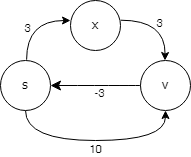
\includegraphics[width=\textwidth]{GrafoPesato01} 
		\caption{Albero di Riccorenza}
	\end{subfigure}
\end{figure} 

Ogni nodo ha due valori:
\begin{itemize}
    \item Dimensione input
    \item Costo locale
\end{itemize}
Ad ogni chiamata sia l'input che il costo vanno a dimezzarsi fino ad arrivare alla foglia che sarà il caso base.

\begin{center}
    \begin{tabular}{||c c||} 
     \hline
     Livello & Contributo \\ [0.5ex] 
     \hline\hline
     0 & n  \\ 
     \hline
     1 & $2*\frac{n}{2} = n$  \\
     \hline
     2 & $4*\frac{n}{4} = n$  \\
     \hline
     \vdots & \vdots \\
     \hline
     i & $2^i*\frac{n}{2^i} = n$ \\ [1ex] 
     \hline
    \end{tabular}
\end{center}



Se andiamo a sommare tutti i contributi di ogni livello dell'albero appena creato avremo che danno tutti lo stesso valore $n$. Grazie a ciò possiamo creare una sommatoria:
$$ T_{MS}(n)=\sum_{i=0}^{?} n$$

Come noteremo la sommatoria dovremmo farla sull'altezza dell'albero, cioè fino a quando l'albero delle chiamate ricorsive arriva al caso base. Sappiamo però che quando incontriamo una foglia, allora allo stesso livello tutte le altre chiamate saranno foglie.\smallskip

Dunque andremo a definire $i$ la nostra altezza incognita.\smallskip

Raccogliamo le informazioni che abbiamo fin ora:

%immagine

Man mano che ci addentriamo nell'albero, la grandezza dell'input diminuisce equamente, e all'ultimo livello avrà formula: $\frac{n}{2^i}$. Però sappiamo che all'ultimo livello, essendo foglia, avremo che la dimensione dell'input e quindi della complessità sarà \textbf{1}.\smallskip

Potremmo quindi impostare un'equazione cosi espressa:

$$\frac{n}{2^i} = 1 \Rightarrow n = 2^i \Rightarrow \log_2 n = \log_2 2^i \Rightarrow \log_2 n = i$$\smallskip

Abbiamo quindi trovato la dimensione di $i$, possiamo quindi sostituirla al punto interrogativo. 

$$ T_{MS}(n)=\sum_{i=0}^{\log_2 n} n \Rightarrow n(\log_2 n+1) = \theta(n\log_2 n)$$
Possiamo dunque approssimare la complessità computazionale di questa equazione di ricorrenza a un caso $n\log_2 n$. 
\smallskip

In questo caso è stato semplice arrivare alla soluzione poichè il valore dell'input fornito ad ogni chiamata ricorsiva è sempre lo stesso e non cambia nel tempo. Potremmo dunque provare a fare un altro esempio andando a cambiare la quantità di chiamate ricorsive ad ogni nodo.

\smallskip

\subsubsection{Esempio 1 con Equazione modificata}

$$T_{MS}(n)= \left\{ \begin{array}{rcl}
    \theta(1) &  n\le1\\
    2 \cdot T(\frac{n}{2})+n^2 & n>1
    \end{array}\right.$$
\smallskip

Andiamo sempre a ragionare come nell'equazione di sopra.

%immagine di valentina che le fa meglio

Come vedremo per ogni livello ora il contributo locale non è piu $n$, ma $n^2$.

In tal senso andiamo a osservare quanto costa ogni livello.

%immagine del costo (tablla)

$$T(n) = \sum_{i=0}^{\log_2 n} \frac{n^2}{2^i} = n^2\sum_{i=0}^{\log_2 n} (\frac{1}{2})^i = n^2 \cdot \theta(1) = \theta(n^2)$$

Il motivo per cui abbiam approssimato a $\theta(1)$ è grazie alla dimostrazione che abbiamo effettuato nelle scorse lezioni. Essendo che 





